\documentclass[12pt]{article}

% Packages
\usepackage[utf8]{inputenc}      % Encoding of the document
\usepackage{graphicx}            % For including images
\usepackage{amsmath, amssymb}    % Math packages
\usepackage{geometry}            % Page layout
\usepackage{hyperref}            % Hyperlinks
\usepackage{natbib}              % Bibliography
\usepackage{caption}             % Custom captions
\usepackage{subcaption}          % Subfigures
\usepackage{listings}            % Code listings
\usepackage{xcolor}              % Colors
\usepackage{biblatex}
\usepackage{tikz}                % Drawing
\usepackage{url}                 % URLs

% Bibliography file:
\addbibresource{bibliography.bib}

% To count pages after the index:
\pagenumbering{gobble}


% Page Layout
\geometry{
    a4paper,
    left=1in,
    right=1in,
    top=1in,
    bottom=1in,
}

% Hyperlink setup
\hypersetup{
    colorlinks=true,
    linkcolor=blue,
    filecolor=magenta,      
    urlcolor=cyan,
}

% Code Listing Style
\lstset{
    language=Python,
    basicstyle=\ttfamily\small,
    keywordstyle=\color{blue},
    commentstyle=\color{gray},
    stringstyle=\color{red},
    numbers=left,
    numberstyle=\tiny\color{gray},
    stepnumber=1,
    numbersep=10pt,
    backgroundcolor=\color{white},
    showspaces=false,
    showstringspaces=false,
    showtabs=false,
    frame=single,
    tabsize=4,
    captionpos=b,
    breaklines=true,
    breakatwhitespace=false,
    escapeinside={\%*}{*)},
}

% Title Information
\title{%
    \vspace{2in} % Adjust vertical space
    \textbf{Tackling the Traveling Salesman Problem with Genetic Algorithms}\\
    \vspace{2in}
}

\author{
    Mauro Vázquez Chas \\
    Dániel Mácsai
    \vspace{0.2in}
}

\date{2024. 11. 10}

\begin{document}

% Title Page
\maketitle
\thispagestyle{empty}

% Abstract
\begin{abstract}
    \noindent
    Abstract goes here.
\end{abstract}

\newpage

\tableofcontents
\newpage



%%%% start counting pages:
\pagenumbering{arabic}

%%%%%%%%%%%%%%%
\section{Introduction}
The Traveling Salesman Problem (TSP) is a classic combinatorial optimization problem that has been extensively studied in the field of mathematics and computer science. The problem is defined as follows: given a set of cities and the distances between them, the goal is to find the shortest possible route that visits each city exactly once and returns to the starting city. The TSP is an NP-hard problem, meaning that there is no known polynomial-time algorithm that can solve it exactly for all instances. In this sense, algorithms such us Genetic Algorithms (GAs) have been proposed as a way to find approximate solutions to the TSP.

\subsection{Dataset}
In this work, we consider a dataset of 29 cities from Bavaria, Germany. The dataset contains the coordinates of each city, as well as the distances between them (provided in a distance matrix). The dataset (called \textit{bays29.tsp}) is available at the following link: \url{http://comopt.ifi.uni-heidelberg.de/software/TSPLIB95/tsp/}


\subsection{Background}
TODO: Provide background information on the topic, including relevant literature and the motivation behind the project.

\subsection{Objectives and scope}
TODO: Outline the main objectives and goals of the project. Define the scope and limitations of the study.



%%%%%%%%%%%%%%%%%%%
\section{Methodology}
\subsection{Problem Representation}
In this work we employed the Pittsburgh view, where each individual in the population represents a complete solution to the TSP. The representation of the problem is a permutation of the cities, where each city is visited exactly once. For example, for a set of cities $\{1,2,3,4\}$, solution $\{1,3,2,4\}$ would represent the path in figure \ref{fig:tsp_example}.

\begin{figure}[h]
    \centering
    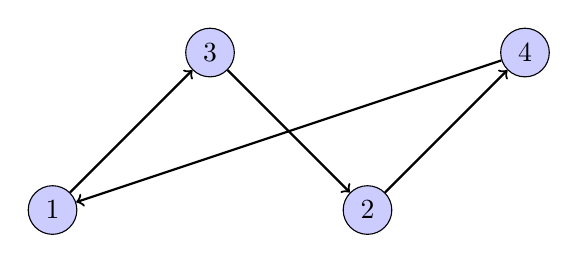
\begin{tikzpicture}
        % Define the nodes
        \node[circle, draw, fill=blue!20] (1) at (0, 0) {1};
        \node[circle, draw, fill=blue!20] (3) at (2, 2) {3};
        \node[circle, draw, fill=blue!20] (2) at (4, 0) {2};
        \node[circle, draw, fill=blue!20] (4) at (6, 2) {4};
        
        % Draw the arrows
        \draw[->, thick] (1) -- (3);
        \draw[->, thick] (3) -- (2);
        \draw[->, thick] (2) -- (4);
        \draw[->, thick] (4) -- (1);
    \end{tikzpicture}
    \caption{Path representation of a TSP solution with nodes 1, 3, 2, and 4.}
    \label{fig:tsp_example}
\end{figure}


We considered different approaches on the representation of each chromosome, either binary code or integer code. Using binary code, each solution would be a string of bits, with each city being a certain number of them. There are variations that use a different encoding mechanism, for example gray encoding. The integer code is a list of integers, where each city is represented by an integer. In the end, we decided to use integer code (called \textit{path representation} in \cite{Larranaga1999}), as it is more intuitive and in binary code, the number of bits used for each city could not be divided. This decision was also influenced by the research made in \cite{Larranaga1999}, where the authors explicitly state the following about binary code :
\begin{quote}
This representation might be useful for small problem instances of the TSP.
However, for larger problem instances the binary strings which represent
the tours become unmanageably large. Another disadvantage of the binary
representation is that the classical operators do not necessarily result in legal
offspring tours; repair algorithms would be necessary.
\end{quote}

In this sense, we are not doing what it is often called canonical or simple genetic algorithm (SGA) as it is described in \cite{Eiben2003}, where the representation is binary. It would be more accurate to say we are using Non-Canonical GAs with integer code representation for each permutation, as they are described in Chapter 17 of \cite{Back2000}.  



\subsection{An overview on Genetic Algorithms}
Genetic Algorithms are, perhaps, the most known evolutionary algorithm. They were pioneered by John Holland in the 1970s, and have since undergone extensive research and numerous adaptations. 

The traditional genetic algorithm, according to \cite{Eiben2003}, uses bit-string representation and works in the following way:
given a population of $\mu$ individuals, we perform the following steps for a certain number of generations:
\begin{enumerate}
    \item Select $\mu$ parents from the population, allowing duplicates
    \item Shuffle the intermediary population and apply crossover and mutation operators to create new individuals
    \item The intermediary population replaces the old population
\end{enumerate}

The selection of the parents is often performed using a selection operator that often requires a fitness function evaluating the quality of the individuals. Classic operators for population modification include bit-flip mutation and one-point crossover.

\subsection{Parent Selection Methods}
Parent selection is a crucial step in the genetic algorithm, as it determines the genetic material that will be passed on to the next generation. In our case, we employed some of the most common mechanisms, according to the material proposed in the lectures \cite{Belanche2024}, and adapting them to the usage of the distance function instead of the fitness function (slightly different as we want to minimize it). The methods used were:
\begin{itemize}
    \item Random selection: parents are selected randomly from the population
    \item Roulette wheel selection: the probability of selecting an individual is proportional to its fitness (in our case, inversely proportional to the distance function)
    \item Rank roulette wheel selection: similar to the previous one, but the probability of selection is proportional to the rank of the individual (in our case, inversely proportional to the rank of the distance function)
    \item Tournament selection: a random subset of the population is selected, and the best individual from this subset is chosen as a parent. We used subsets of size 3 and 5.
\end{itemize}


\subsection{Crossover techniques}
TODO:Describe the POS operator, its implementation, and its role in the genetic algorithm.
/cite{Larranaga1999}

\subsection{Mutation Operators}
The mutation operator is a crucial part of the genetic algorithm, as it introduces diversity into the population. For reference, we checked \cite{Larranaga1999}. In the end, in our implementation, we used the following mutation operators:
\begin{itemize}
    \item Exchange mutation: two random cities are arbitrarily swapped in the chromosome
    \item Insertion mutation: a random city is removed and reinserted at another random position in the chromosome
    \item TODO: Inversion mutation: a subset of the chromosome is reversed
\end{itemize}

\subsection{Elitism}
Elitism is a mechanism that ensures that the best individuals from the current population are passed on to the next generation. This helps maintain the best solutions found so far and prevents the degradation of chromosome quality. In our implementation, we considered GA configurations without elitism and with elitism, both keeping the best individual and the three best individuals from the previous generation.

\subsection{Other Considered Approaches}
\subsubsection{Fitness Function}
As we already noted, we employed the total distance of the path as the value to optimize, to minimize if we want to be precise. However, the common approach would be to use a fitness function, were better chromosomes have higher values. In this sense, we could have used any monotonic decreasing function of the distance, for example, the reciprocal of the distance or a decaying exponential function. This would have allowed us to use the classic selection operators without modifications. However, we decided to use the distance directly, as it is more intuitive and straightforward.

\subsubsection{Population Replacement}
In this work we used a generational approach, where the entire population is replaced at each generation $(\mu,\lambda), \mu=\lambda$. However, we also considered a steady-state approach where only a subset of the population is replaced at each generation. Ultimately we decided not to do this, as it would have required a more complex implementation and in words of \cite{Eiben2003}: "It can also lead to premature convergece as the population tends to rapidly focus on the fittest member". 

A useful follow-up of this work would be to implement a steady-state approach by inverse tournament selection as it doesn't remove as much genetic diversity, due to its innate randomness.

Even though we described our implementation as $(\mu,\lambda), \mu=\lambda$, it could be seen as a $(\mu,\lambda), \mu>\lambda$ approach when we make use of elitism, as we keep the best individuals from the previous generation and $\mu=\lambda+\text{elitism}$.


\subsubsection{Population Initialization}
We evaluated different ways to initialize the population, including random initialization (the one we opted for) and heuristic initialization. This last one, refers to the usage of a heuristic algorithm to generate the initial population. This could be useful for large instances of the TSP, as it would provide a good starting point for the genetic algorithm. The practice is commented in Chapter 13 of \cite{Back2000}, where the authors also explore the hybridization of evolutionary strategies with domain specific knowledge and algorithms, highlighting the good results of the available literature.

However, we decided not to implement this, as it would require the usage of a heuristic algorithm and other techniques that are out of the scope of this work. Having said this, it would be interesting to further explore this.

\subsubsection{Other Operators}
TODO: Write about some options and the reasons why we didn't use them. (computational time of the grid search, etc.)

% Implementation
\section{Implementation}
\subsection{Environment Setup}
One of our main goals, was to create a flexible and modular implementation that allows for easy experimentation with different configurations and operators. To achieve this, we used Python as the main programming language, and we implemented the parent-selection methods, crossover operators, and mutation operators as separate modules. This design allows us to easily swap out different operators and configurations without changing the core logic of the genetic algorithm. Aside from this, the class that contains the genetic algorithm is also modular, allowing for easy extension and modification. All of these files, can be found in the \textit{src} folder of the project.

Another clear target of ours, was to code (almost) everything from scratch. For this reason, we only used the following libraries:
\begin{enumerate}
    \item \textit{numpy} for numerical operations and efficiency
    \item \textit{random} for random number generation
    \item \textit{matplotlib} for visualization
    \item \textit{typing} for type hints
    \item \textit{logging} for better debugging
    \item \textit{json} to save the results
    \item \textit{datetime} to save the results
    \item \textit{pandas} to deal with the results in a more structured way for the analysis
\end{enumerate}

To use all of these modules, we set up a jupyter notebook file \textit{tsp.ipynb} that contains the data reading function, the grid search function and most graph plotting cells. In this notebook, we also wrote a \textit{Usage Example} section, where we show how to use the genetic algorithm class and all of its parameters, although if more insight is needed, all the functions and classes are documented in their respective docstrings.

\subsection{Code Structure}

\begin{figure}
    \centering
    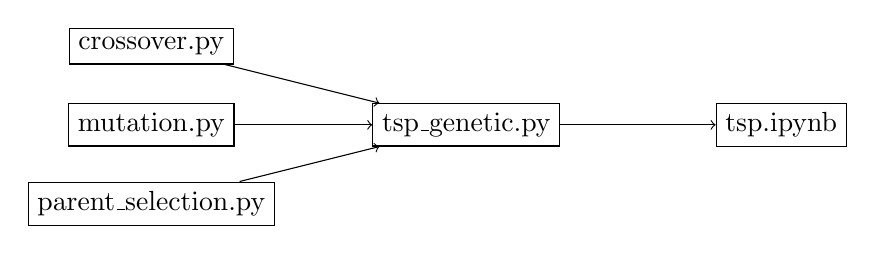
\begin{tikzpicture}[node distance=1cm, auto]
        % Nodes
        \node (crossover) [draw, rectangle] {crossover.py};
        \node (mutation) [draw, rectangle, below of=crossover] {mutation.py};
        \node (parent_selection) [draw, rectangle, below of=mutation] {parent\_selection.py};
        \node (tsp_genetic) [draw, rectangle, right of=mutation, node distance=4cm] {tsp\_genetic.py};
        \node (tsp_notebook) [draw, rectangle, right of=tsp_genetic, node distance=4cm] {tsp.ipynb};

        % Arrows
        \draw[->] (crossover) -- (tsp_genetic);
        \draw[->] (mutation) -- (tsp_genetic);
        \draw[->] (parent_selection) -- (tsp_genetic);
        \draw[->] (tsp_genetic) -- (tsp_notebook);
    \end{tikzpicture}
    \caption{Code Structure Diagram}
    \label{fig:code_structure}
\end{figure}


Provide an overview of the code structure, including key modules and their functionalities. 

\subsection{Key Algorithms}
Include code snippets and explanations of the core algorithms implemented. 

\subsubsection{Position-Based Crossover}


% Results
\section{Results}
\subsection{Experimental Setup}
Describe the experiments conducted, including parameters and datasets used.


The number of configurations considered was: 3240
The best chromosome found was: [11  8  4 25 28  2  1 20  0  7 26 22  6 24 18 10 21 13 16 17 14  3 19  9
 12 15 23 27  5]
The best distance found was: 2055.0
The best parameters were: {'population_size': 200, 'elitism': 1, 'generations': 200, 'm_rate': 0.1, 'c_rate': 1, 'select_parents': 'tournament_selection', 'crossover': 'POS', 'mutation': 'insertion', 'tournament_size': 5}


\subsection{Performance Analysis}
Present and analyze the results, using figures and tables as necessary.

\subsection{Discussion}
Interpret the results, discussing their implications and any observed patterns.

% Conclusion
\section{Conclusion}
\subsection{Summary}
Summarize the key findings and contributions of the project.

\subsection{Future Work}
Suggest potential areas for future research or improvements.

% References
\newpage
\printbibliography

% Appendix
\appendix
\chapter{Appendix A}
Include any supplementary material, such as additional code or data.

\end{document}